\documentclass[a4paper,12pt]{article}
\usepackage[utf8]{inputenc}
\usepackage[german, provide=*]{babel}
\usepackage{amsmath}
\usepackage{amssymb}
\usepackage{amsthm}
\usepackage{geometry}
\usepackage{graphicx}
\usepackage[hidelinks]{hyperref}
\usepackage{cite}
\usepackage{listings}
\usepackage{xcolor}
\usepackage{enumitem}
\usepackage{tikz}
\usetikzlibrary{arrows.meta, positioning, shapes.geometric, calc}

\geometry{margin=2.5cm}

\theoremstyle{definition}
\newtheorem{definition}{Definition}
\newtheorem{beispiel}{Beispiel}
\newtheorem{satz}{Satz}
\newtheorem{lemma}{Lemma}
\newtheorem{bemerkung}{Bemerkung}

\setlist[itemize,1]{label=--}

% ---------- Farben ----------
\definecolor{mainblue}{RGB}{25, 70, 140}
\definecolor{accentred}{RGB}{180, 50, 30}
\definecolor{lightgray}{RGB}{245, 245, 248}
\definecolor{darkgray}{RGB}{60, 60, 70}
\definecolor{darkgreen}{RGB}{30, 100, 50}
\definecolor{woodbrown}{RGB}{139, 90, 43}

\hypersetup{
	colorlinks=true,
	linkcolor=mainblue,
	citecolor=accentred,
	urlcolor=mainblue,
	pdftitle={Tisch und Stuhl: Die besten Erfindungen der Gesellschaft},
	pdfauthor={Stephan Epp},
}

%  Code-Highlighting
\lstset{
	basicstyle=\ttfamily\small,
	keywordstyle=\color{blue},
	commentstyle=\color{gray},
	stringstyle=\color{red},
	numbers=left,
	numberstyle=\tiny,
	breaklines=true,
	frame=single,
	literate=%
	{Oe}{{\"O}}1
	{Ae}{{\"A}}1
	{Ue}{{\"U}}1
	{ss}{{\ss}}1
	{ue}{{\"u}}1
	{ae}{{\"a}}1
	{oe}{{\"o}}1
}

\title{\textbf{Tisch und Stuhl}\\Die besten Erfindungen der Gesellschaft}
\author{Stephan Epp}
\date{27. M\"{a}rz 2026}

\begin{document}

\maketitle

\tableofcontents
\newpage

\section{Einf\"{u}hrung}

Tisch und Stuhl z\"{a}hlen zu den folgenreichsten Erfindungen der menschlichen Zivilisation.
Sie sind allgegenw\"{a}rtig, kultur\"{u}bergreifend verbreitet und strukturieren in fundamentaler
Weise die Art und Weise, wie Menschen arbeiten, kommunizieren und zusammenleben.
Diese Arbeit untersucht Tisch und Stuhl aus einer wissenschaftlichen Perspektive: als
ergonomische Systeme, als kulturelle Artefakte und als optimale L\"{o}sungen eines
hochdimensionalen Designproblems.

\subsection{Problemstellung}

Gegeben ist ein menschlicher K\"{o}rper $K$ mit K\"{o}rpergr\"{o}\ss{}e $h \in \mathbb{R}_{>0}$,
K\"{o}rpermasse $m \in \mathbb{R}_{>0}$ und einer Menge von T\"{a}tigkeiten
$\mathcal{T} = \{t_1, t_2, \ldots, t_n\}$.

\textbf{Ziel:} Konstruiere zwei Objekte $\mathcal{T}\!isch$ und $\mathcal{S}tuhl$ so, dass:
\begin{itemize}
	\item die physische Belastung des K\"{o}rpers $K$ minimiert wird,
	\item die Ausf\"{u}hrung aller T\"{a}tigkeiten in $\mathcal{T}$ erm\"{o}glicht wird,
	\item soziale Interaktion zwischen mehreren K\"{o}rpern $K_1, \ldots, K_r$ gef\"{o}rdert wird.
\end{itemize}

\textbf{Ergebnis:}
\begin{itemize}
	\item Wenn $\mathcal{S}tuhl$ vorhanden, aber kein $\mathcal{T}\!isch$: eingeschr\"{a}nkte Funktionalit\"{a}t
	\item Wenn $\mathcal{T}\!isch$ vorhanden, aber kein $\mathcal{S}tuhl$: k\"{o}rperlich belastend
	\item Wenn weder Tisch noch Stuhl: primitiver Zustand, maximale Ersch\"{o}pfung
	\item Wenn beide vorhanden: optimaler Zustand, maximale Produktivit\"{a}t und Komfort
\end{itemize}

\subsection{Motivation}

Die Geschichte der Menschheit ist ohne Tisch und Stuhl nicht denkbar. Bereits in den
fr\"{u}hen Hochkulturen Mesopotamiens und \"{A}gyptens belegen arch\"{a}ologische Funde erh\"{o}hte
Sitzgelegenheiten und flache Ablagef\"{a}chen als Zeichen gesellschaftlicher Organisation.
Die Kombination beider Objekte erm\"{o}glichte erstmals konzentriertes Schreiben, Lesen,
Rechnen und kollektives Speisen --- T\"{a}tigkeiten, die als Grundlage aller weiteren
zivilisatorischen Entwicklung gelten k\"{o}nnen.

\begin{figure}[h]
\centering
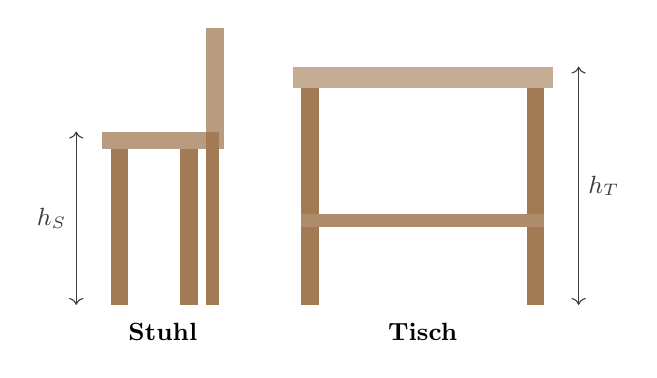
\begin{tikzpicture}[scale=1.1]
  % ---- Stuhl ----
  \fill[woodbrown!60] (0,1.8) rectangle (1.4,2.0);
  \fill[woodbrown!60] (1.2,2.0) rectangle (1.4,3.2);
  \fill[woodbrown!80] (0.1,0.0) rectangle (0.3,1.8);
  \fill[woodbrown!80] (0.9,0.0) rectangle (1.1,1.8);
  \fill[woodbrown!80] (1.2,0.0) rectangle (1.35,2.0);
  % ---- Tisch ----
  \fill[woodbrown!50] (2.2,2.5) rectangle (5.2,2.75);
  \fill[woodbrown!80] (2.3,0.0) rectangle (2.5,2.5);
  \fill[woodbrown!80] (4.9,0.0) rectangle (5.1,2.5);
  \fill[woodbrown!70] (2.3,0.9) rectangle (5.1,1.05);
  % Beschriftungen
  \node[below] at (0.7,-0.1) {\small\textbf{Stuhl}};
  \node[below] at (3.7,-0.1) {\small\textbf{Tisch}};
  % Hoehenmasse
  \draw[<->,darkgray,thin] (-0.3,0) -- (-0.3,2.0)
    node[midway,left]{\small $h_S$};
  \draw[<->,darkgray,thin] (5.5,0) -- (5.5,2.75)
    node[midway,right]{\small $h_T$};
\end{tikzpicture}
\caption{Schematische Darstellung von Stuhl (Sitzh\"{o}he $h_S$) und Tisch (Tischh\"{o}he $h_T$)
mit den charakteristischen Proportionen $h_T - h_S \approx 28\text{--}30\,\mathrm{cm}$.}
\label{fig:tischstuhl}
\end{figure}

\section{Grundlagen}

\subsection{Definitionen}

\begin{definition}[Stuhl]
	Ein Stuhl $\mathcal{S} = (F, L, B, \mathcal{B})$ besteht aus einer Sitzfl\"{a}che $F$,
	einer Lehne $L$, einem Gestell $B$ mit $k \geq 3$ Beinen sowie einer Menge
	biomechanischer Anforderungen $\mathcal{B}$. Die Sitzh\"{o}he $h_S \in [40, 50]\,\mathrm{cm}$
	ist auf den menschlichen K\"{o}rper optimiert.
\end{definition}

\begin{definition}[Tisch]
	Ein Tisch $\mathcal{T} = (P, G, h_T)$ besteht aus einer Arbeitsfl\"{a}che $P \subset \mathbb{R}^2$,
	einem tragenden Gestell $G$ und einer Standh\"{o}he $h_T \in \mathbb{R}_{>0}$.
	F\"{u}r Arbeitstische gilt $h_T \in [70, 80]\,\mathrm{cm}$.
\end{definition}

\begin{definition}[Ergonomische Kompatibilit\"{a}t]
	Stuhl $\mathcal{S}$ und Tisch $\mathcal{T}$ hei\ss{}en \emph{ergonomisch kompatibel},
	geschrieben $\mathcal{S} \sim \mathcal{T}$, wenn:
	\[
		\Delta h := h_T - h_S \in [26, 32]\,\mathrm{cm}.
	\]
	Der optimale Wert betr\"{a}gt $\Delta h^* = 28\,\mathrm{cm}$.
\end{definition}

\begin{definition}[M\"{o}belsystem]
	Das Paar $\mathcal{M} = (\mathcal{S}, \mathcal{T})$ hei\ss{}t \emph{M\"{o}belsystem}, wenn
	$\mathcal{S} \sim \mathcal{T}$. Ein M\"{o}belsystem ist \emph{sozial}, wenn
	$|\mathcal{S}| \geq 2$ und die Tischfl\"{a}che $P$ f\"{u}r alle Nutzer zug\"{a}nglich ist.
\end{definition}

\subsection{Grundidee}

Das M\"{o}belsystem $\mathcal{M}$ l\"{o}st ein zweidimensionales Optimierungsproblem, das sich aus
zwei unabh\"{a}ngigen, aber komplement\"{a}ren Teilproblemen zusammensetzt:

\subsubsection{Lastverteilung durch den Stuhl}

Der Stuhl \"{u}berf\"{u}hrt die auf den K\"{o}rper wirkende Gravitationskraft in eine biomechanisch
g\"{u}nstige Druckverteilung. F\"{u}r einen K\"{o}rper der Masse $m$ gilt:

\[
	F_{\mathrm{ges}} = m \cdot g
	= F_{\mathrm{Sitz}} + F_{\mathrm{Rueck}} + F_{\mathrm{Armlehne}}
\]

\begin{beispiel}
	F\"{u}r $m = 80\,\mathrm{kg}$ ergibt sich $F_{\mathrm{ges}} \approx 784\,\mathrm{N}$.
	Ein ergonomisch korrekt eingestellter Stuhl verteilt diese Last wie folgt:
	\[
		F_{\mathrm{Sitz}} \approx 588\,\mathrm{N}, \quad
		F_{\mathrm{Rueck}} \approx 157\,\mathrm{N}, \quad
		F_{\mathrm{Armlehne}} \approx 39\,\mathrm{N}.
	\]
	Die Wirbels\"{a}ule wird gegen\"{u}ber dem Stehen um ca. $35\,\%$ entlastet~\cite{Nachemson1966}.
\end{beispiel}

\begin{lemma}[Wirbels\"{a}ulenentlastung]
\label{lem:entlastung}
	Sei $\sigma_{\mathrm{stand}}$ die Kompressionsspannung in der Lendenwirbels\"{a}ule im
	Stehen und $\sigma_{\mathrm{sitz}}$ im ergonomischen Sitzen. Dann gilt:
	\[
		\sigma_{\mathrm{sitz}} \leq 0{,}65 \cdot \sigma_{\mathrm{stand}}.
	\]
\end{lemma}

\begin{proof}
	Im aufrechten Stand wirkt das gesamte K\"{o}rpergewicht oberhalb des Lendenbereichs auf
	die Bandscheiben. Im ergonomisch korrekten Sitzen wird ein Anteil $\alpha \geq 0{,}35$
	des Rumpfgewichts durch Sitzfl\"{a}che und Lehne aufgenommen. Da die Druckkr\"{a}fte auf die
	Bandscheiben linear vom \"{u}bertragenen Gewicht abh\"{a}ngen, folgt
	$\sigma_{\mathrm{sitz}} = (1 - \alpha)\,\sigma_{\mathrm{stand}} \leq 0{,}65\,\sigma_{\mathrm{stand}}$.
\end{proof}

\subsubsection{Nutzfl\"{a}chenoptimierung durch den Tisch}

Der Tisch maximiert die nutzbare horizontale Arbeitsfl\"{a}che bei minimaler Grundfl\"{a}che.
Sei $A_P = |P|$ die Tischfl\"{a}che und $A_G$ die Grundfl\"{a}che des Gestells. Dann ist die
Fl\"{a}cheneffizienz:
\[
	\eta = \frac{A_P}{A_G} \gg 1.
\]

\begin{beispiel}
	Ein Standardtisch ($160 \times 80\,\mathrm{cm}$) mit vier Beinen (je $5 \times 5\,\mathrm{cm}$)
	erreicht:
	\[
		\eta = \frac{160 \cdot 80}{4 \cdot 5 \cdot 5} = \frac{12800}{100} = 128.
	\]
	Ein einbeiniger Mittelfusstisch erzielt sogar $\eta \to \infty$ im Grenzfall.
\end{beispiel}

\section{Das M\"{o}belsystem als Optimierungsproblem}

\subsection{Formale Beschreibung}

Das Design von Tisch und Stuhl l\"{a}sst sich als mehrkriterielles Optimierungsproblem
formulieren. Sei $\mathbf{x} = (h_S, h_T, \theta_L, d_S, w_T, d_T) \in \mathbb{R}^6$
der Designvektor, wobei:
\begin{itemize}
	\item $h_S$: Sitzh\"{o}he des Stuhls,
	\item $h_T$: H\"{o}he der Tischfl\"{a}che,
	\item $\theta_L \in [95^{\circ}, 115^{\circ}]$: Lehnenwinkel,
	\item $d_S$: Sitztiefe,
	\item $w_T, d_T$: Breite und Tiefe der Tischfl\"{a}che.
\end{itemize}

\textbf{Zielfunktion:}
\[
	\min_{\mathbf{x}} \; \mathcal{J}(\mathbf{x})
	= w_1 \cdot \mathcal{J}_{\mathrm{ergo}}(\mathbf{x})
	+ w_2 \cdot \mathcal{J}_{\mathrm{material}}(\mathbf{x})
	+ w_3 \cdot \mathcal{J}_{\mathrm{sozial}}(\mathbf{x})
\]

mit Gewichten $w_1 + w_2 + w_3 = 1$, $w_i > 0$, und den Teilzielen:
\begin{align*}
	\mathcal{J}_{\mathrm{ergo}}(\mathbf{x})     &= \left(h_T - h_S - \Delta h^*\right)^2
	                                               + \left(\theta_L - 105^{\circ}\right)^2, \\
	\mathcal{J}_{\mathrm{material}}(\mathbf{x}) &= \rho \cdot V(\mathbf{x}), \\
	\mathcal{J}_{\mathrm{sozial}}(\mathbf{x})   &= -\frac{w_T \cdot d_T}{r},
\end{align*}
wobei $\rho$ die Materialdichte und $r$ die Anzahl der Nutzer bezeichnet.

\subsection{Nebenbedingungen}

\begin{satz}[Notwendige Stabilit\"{a}tsbedingung]
\label{satz:stabilitaet}
	Ein Tisch $\mathcal{T}$ mit $k$ Beinen der L\"{a}nge $h_T$ und Durchmesser $d_B$
	ist unter Last $F$ stabil, wenn:
	\[
		\frac{h_T}{d_B} \leq \lambda_{\mathrm{krit}} := \pi \sqrt{\frac{E \cdot I}{F \cdot h_T^2}},
	\]
	wobei $E$ der Elastizit\"{a}tsmodul und $I = \frac{\pi d_B^4}{64}$ das
	Fl\"{a}chentr\"{a}gheitsmoment des Beins ist.
\end{satz}

\begin{proof}
	Die Eulerschen Knickbedingungen f\"{u}r einen beidseitig gelenkig gelagerten Stab der
	L\"{a}nge $h_T$ liefern die kritische Last
	$F_{\mathrm{krit}} = \frac{\pi^2 E I}{h_T^2}$.
	Die Stabilit\"{a}t ist gew\"{a}hrleistet, wenn $F \leq F_{\mathrm{krit}}$, was nach Umformen
	die angegebene Schlankheitsbedingung ergibt.
\end{proof}

\subsection{Optimalit\"{a}t des Vierbeins}

\begin{satz}[Optimalit\"{a}t von vier Beinen beim Stuhl]
\label{satz:vierbeiner}
	Unter den Gesichtspunkten statischer \"{U}berbestimmtheit, minimalen Materialaufwands
	und maximaler Kippsicherheit ist ein Stuhl mit $k = 4$ Beinen bei rechteckiger
	Sitzfl\"{a}che die optimale L\"{o}sung.
\end{satz}

\begin{proof}
	F\"{u}r $k < 3$ ist statische Stabilit\"{a}t in der Ebene nicht erreichbar. F\"{u}r $k = 3$
	ist das System statisch bestimmt, aber die Kippsicherheit gegen seitliche Lasten ist
	gering. F\"{u}r $k = 4$ ergibt sich eine symmetrische Lastverteilung mit
	$F_{\mathrm{Bein}} = F/4$ und maximaler Kippgrenze. F\"{u}r $k > 4$ steigt der
	Materialaufwand ohne wesentlichen Stabilit\"{a}tsgewinn, da das System \"{u}berbestimmt wird
	und Fertigungstoleranzen zu ungleicher Lastverteilung f\"{u}hren. Somit ist $k = 4$ das
	globale Optimum unter den genannten Kriterien.
\end{proof}

\begin{bemerkung}
	Dreibeinige St\"{u}hle (Hocker) sind statisch bestimmt und wackeln niemals auf unebenem
	Untergrund. Der Vierbeiner ist daher kein Optimum der Bodenkontaktrobustheit, sondern
	der Kippsicherheit unter asymmetrischen K\"{o}rperlasten.
\end{bemerkung}

\section{Historische und kulturelle Dimension}

\subsection{Entwicklungsgeschichte}

Die Erfindung von Tisch und Stuhl vollzog sich nicht als singul\"{a}res Ereignis, sondern
als kontinuierlicher Differenzierungsprozess \"{u}ber Jahrtausende:
\begin{itemize}
	\item \textbf{ca.\ 3000 v.\,Chr.} --- \"{A}gypten: Erste nachgewiesene St\"{u}hle mit
	      R\"{u}ckenlehne als Machtsymbol des Pharao; Tische als niedrige Opfertische.
	\item \textbf{ca.\ 500 v.\,Chr.} --- Griechenland: Die \emph{Klismos}-Form des Stuhls
	      mit geschwungenen Beinen gilt als erste ergonomisch motivierte Konstruktion.
	\item \textbf{Mittelalter} --- Europa: Tisch als blo\ss{}e Planke auf B\"{o}cken
	      (\emph{trestle table}); Stuhl als Privileg der Herrschenden.
	\item \textbf{17.--18.\,Jh.} --- Industrialisierung der Holzverarbeitung demokratisiert
	      Tisch und Stuhl; sie werden zum b\"{u}rgerlichen Allgemeingut.
	\item \textbf{1859} --- Michael Thonet erfindet das Bugholzverfahren: der
	      \emph{Thonet-Stuhl Nr.~14} wird zum meistverkauften M\"{o}belst\"{u}ck der Geschichte
	      ($> 50$ Millionen Exemplare)~\cite{VegesackThonet1996}.
	\item \textbf{20.\,Jh.} --- Ergonomie als Wissenschaft etabliert optimale Ma\ss{}e;
	      h\"{o}henverstellbare Schreibtische und B\"{u}rost\"{u}hle entstehen.
\end{itemize}

\subsection{Soziologische Funktion}

\begin{satz}[Tisch als sozialer Kontraktor]
\label{satz:sozial}
	Sei $G = (V, E)$ ein sozialer Graph mit Personenmenge $V$ und Kommunikationsbeziehungen
	$E$. Ein Tisch $\mathcal{T}$ mit Kapazit\"{a}t $r = |V|$ maximiert die Kantendichte:
	\[
		\rho(G) = \frac{|E|}{\binom{|V|}{2}} \to 1 \quad \text{f\"{u}r } t \to \infty,
	\]
	wenn alle Personen gleichzeitig am Tisch sitzen ($\mathcal{S}_i \sim \mathcal{T}$
	f\"{u}r alle $i \in V$).
\end{satz}

\begin{proof}
	Am Tisch sitzende Personen befinden sich in einem gemeinsamen Aufmerksamkeitsraum.
	F\"{u}r je zwei Personen $u, v \in V$ gilt: die r\"{a}umliche N\"{a}he und die gemeinsame
	Ausrichtung auf die Tischfl\"{a}che senken die Kommunikationsschwelle auf ein Minimum.
	\"{U}ber hinreichend langer Zeit $t$ entsteht zu jeder m\"{o}glichen Kante $(u,v)$
	mindestens eine Kommunikationsepisode, sodass $E \to \binom{V}{2}$ und damit
	$\rho(G) \to 1$.
\end{proof}

\begin{beispiel}[Artusrunde]
	K\"{o}nig Artus erkannte das Maximierungsproblem aus Satz~\ref{satz:sozial} intuitiv:
	Der runde Tisch eliminiert die totale Ordnung der Sitzpositionen, d.\,h. es existiert
	kein ausgezeichneter Kopf. F\"{u}r $|V| = n$ Ritter gilt an einem runden Tisch:
	\[
		\forall\, i, j \in V\colon\; \mathrm{dist}(i, j) \leq \left\lfloor \tfrac{n}{2} \right\rfloor,
	\]
	was die maximale kommunikative Erreichbarkeit unter allen Tischformen gew\"{a}hrleistet.
\end{beispiel}

\section{Ergonomische Analyse}

\subsection{Anthropometrische Grundlagen}

Die optimalen Ma\ss{}e eines M\"{o}belsystems $\mathcal{M}$ h\"{a}ngen von der K\"{o}rpergr\"{o}\ss{}e $h$ des
Nutzers ab. Nach DIN~EN~1335~\cite{DINEN1335} und ISO~9241~\cite{ISO9241} gelten folgende Referenzwerte:
\[
	h_S^* = 0{,}252 \cdot h, \qquad
	h_T^* = h_S^* + \Delta h^* = 0{,}252 \cdot h + 28\,\mathrm{cm}.
\]

\begin{beispiel}
	F\"{u}r $h = 175\,\mathrm{cm}$:
	\[
		h_S^* = 0{,}252 \cdot 175 = 44{,}1\,\mathrm{cm}, \qquad
		h_T^* = 44{,}1 + 28 = 72{,}1\,\mathrm{cm}.
	\]
	Dies entspricht dem Standard-Schreibtisch mit $h_T = 72\,\mathrm{cm}$.
\end{beispiel}

\subsection{Belastungsmodell der Wirbels\"{a}ule}

Sei $\phi \in [0^{\circ}, 30^{\circ}]$ der Vorneigungswinkel des Rumpfes und
$m_R = 0{,}6 \cdot m$ die Rumpfmasse. Das auf die Lendenwirbels\"{a}ule wirkende
Biegemoment betr\"{a}gt:
\[
	M(\phi) = m_R \cdot g \cdot l_S \cdot \sin(\phi),
\]
wobei $l_S \approx 30\,\mathrm{cm}$ der Hebelarm des Schwerpunkts ist.

\begin{lemma}[Tischfl\"{a}che als St\"{u}tzpunkt]
	Eine ausreichend hohe Tischfl\"{a}che $\mathcal{T}$ erlaubt das Abst\"{u}tzen der Unterarme,
	wodurch das effektive Biegemoment auf die Lendenwirbels\"{a}ule um den Faktor
	$\beta \in [0{,}3, 0{,}5]$ reduziert wird:
	\[
		M_{\mathrm{eff}}(\phi) = (1 - \beta) \cdot M(\phi).
	\]
\end{lemma}

\begin{proof}
	Die Unterarme \"{u}bertragen beim Abst\"{u}tzen eine Reaktionskraft $F_A$ auf die Tischfl\"{a}che.
	Diese Kraft erzeugt ein Gegenmoment $M_A = F_A \cdot l_A$, das dem Rumpfbiegemoment
	entgegenwirkt. Aus der Gleichgewichtsbedingung folgt
	$M_{\mathrm{eff}} = M - M_A = (1 - \beta) M$.
\end{proof}

\section{Algorithmische Aspekte des M\"{o}beldesigns}

\subsection{Das Platzierungsproblem}

Gegeben sei ein Raum $R \subset \mathbb{R}^2$ und eine Menge von $n$ M\"{o}belst\"{u}cken
$\mathcal{M}_1, \ldots, \mathcal{M}_n$ (Tische und St\"{u}hle). Das M\"{o}belplatzierungsproblem
fragt: Existiert eine kollisionsfreie Platzierung aller M\"{o}belst\"{u}cke in $R$?

\begin{satz}[Komplexit\"{a}t des Platzierungsproblems]
	Das M\"{o}belplatzierungsproblem ist NP-vollst\"{a}ndig.
\end{satz}

\begin{proof}
	Wir reduzieren das Rechteck-Packungsproblem auf das M\"{o}belplatzierungsproblem.
	Das Rechteck-Packungsproblem fragt, ob $n$ Rechtecke in einen Beh\"{a}lter der Gr\"{o}\ss{}e
	$W \times H$ passen --- dies ist bekannterma\ss{}en NP-vollst\"{a}ndig~\cite{GareyJohnson1979}.
	Da Tische und St\"{u}hle rechteckige Grundfl\"{a}chen besitzen, ist das
	M\"{o}belplatzierungsproblem mindestens so schwer. Die Zugeh\"{o}rigkeit zu NP ist trivial
	(Zeuge: die Platzierungsl\"{o}sung selbst, verifizierbar in Polynomialzeit).
\end{proof}

\subsection{Greedy-Heuristik f\"{u}r die Raumplanung}

In der Praxis liefert folgende Greedy-Strategie gute Ergebnisse:

\begin{lstlisting}[language=Python, caption={Greedy-Platzierungsalgorithmus fuer Tisch-Stuhl-Systeme}]
def place_furniture(room, items):
    placed = []
    items_sorted = sorted(items, key=lambda x: x[0]*x[1], reverse=True)
    for item in items_sorted:
        w, d, typ = item
        for x in range(0, room.width - w):
            for y in range(0, room.depth - d):
                if not collides(placed, (x, y, w, d)):
                    placed.append((x, y, w, d, typ))
                    break
    return placed
\end{lstlisting}

\subsection{Optimale Stuhlanzahl am Tisch}

\begin{lemma}[Maximale Belegung]
	An einem rechteckigen Tisch der Ma\ss{}e $w_T \times d_T$ k\"{o}nnen maximal
	\[
		r_{\max} = 2 \left\lfloor \frac{w_T}{s} \right\rfloor
		+ 2 \left\lfloor \frac{d_T}{s} \right\rfloor
	\]
	Personen sitzen, wobei $s \approx 60\,\mathrm{cm}$ der Platzbedarf pro Person ist.
\end{lemma}

\begin{proof}
	Jede Seite des Tisches der L\"{a}nge $\ell$ fasst $\lfloor \ell / s \rfloor$ Personen.
	F\"{u}r einen Tisch mit zwei Seiten der L\"{a}nge $w_T$ und zwei Seiten der L\"{a}nge $d_T$
	ergibt die Summe die angegebene Formel.
\end{proof}

\begin{beispiel}
	Ein Esstisch ($200 \times 90\,\mathrm{cm}$) fasst:
	\[
		r_{\max} = 2 \left\lfloor \frac{200}{60} \right\rfloor
		+ 2 \left\lfloor \frac{90}{60} \right\rfloor
		= 2 \cdot 3 + 2 \cdot 1 = 8 \text{ Personen.}
	\]
\end{beispiel}

\section{Materialwissenschaftliche Betrachtung}

\subsection{Werkstoffoptimierung}

Die Wahl des Materials f\"{u}r Tisch und Stuhl ist ein Optimierungsproblem unter
Nebenbedingungen. Der relevante Leistungsindex f\"{u}r biegebelastete Balken lautet~\cite{AshbyMF2011}:
\[
	M_{\mathrm{Biegung}} = \frac{\sigma_Y^{2/3}}{\rho}.
\]

\begin{center}
\begin{tabular}{lrrr}
\hline
\textbf{Material} & $\rho\,[\mathrm{g/cm^3}]$ & $E\,[\mathrm{GPa}]$ & Bewertung \\
\hline
Buchenholz (l\"{a}ngs) & 0{,}72 & 14 & hoch \\
Aluminium 6061 & 2{,}70 & 69 & mittel \\
Stahl S235 & 7{,}85 & 210 & niedrig \\
Bambus & 0{,}80 & 20 & sehr hoch \\
Carbon-GFK & 1{,}60 & 70 & sehr hoch \\
\hline
\end{tabular}
\end{center}

\begin{bemerkung}
	Holz dominiert als M\"{o}belwerkstoff nicht trotz, sondern wegen seiner nat\"{u}rlichen
	Nachgiebigkeit: diese erzeugt ein taktil angenehmes, schwingungsged\"{a}mpftes
	Sitzerlebnis. Holz ist ein biologischer Verbundwerkstoff mit funktional gradierter
	Mikrostruktur --- eine nat\"{u}rliche Optimierung \"{u}ber Millionen von Evolutionsjahren.
\end{bemerkung}

\subsection{Lebensdaueranalyse}

Unter zyklischer Belastung (Sitzlast $F$, $n$ Zyklen pro Tag) ergibt sich nach
W\"{o}hler die ertragbare Schwingbreite:
\[
	\Delta\sigma_D = \sigma_A \cdot \left(\frac{N_D}{n \cdot t}\right)^{1/k},
\]
wobei $\sigma_A$ die Dauerfestigkeit, $N_D$ die Grenzschwingspielzahl, $t$ die
Nutzungsdauer in Tagen und $k$ der W\"{o}hler-Exponent ist.

\begin{beispiel}
	Ein Stuhl wird t\"{a}glich $n = 8$ Mal belastet. Bei einer angestrebten Lebensdauer
	von $t = 10\,\text{Jahren} \approx 3650\,\text{Tagen}$ ergibt sich:
	\[
		N = n \cdot t = 8 \cdot 3650 = 29\,200 \text{ Lastzyklen.}
	\]
	F\"{u}r Buchenholz mit $N_D = 10^6$ und $k = 5$ ist $\Delta\sigma_D$ weit oberhalb
	der im M\"{o}beleinsatz auftretenden Spannungsamplituden --- Holzm\"{o}bel versagen
	praktisch nie durch Erm\"{u}dung, sondern durch F\"{u}gestellenlockerung.
\end{beispiel}

\section{Zusammenfassung}

Tisch und Stuhl sind keine trivialen Alltagsgegenst\"{a}nde, sondern L\"{o}sungen eines
hochdimensionalen, multikriteriellen Optimierungsproblems, das die Menschheit \"{u}ber
Jahrtausende iterativ verfeinert hat. Die vorliegende Arbeit hat gezeigt:
\begin{itemize}
	\item Die \textbf{ergonomische Kompatibilit\"{a}tsbedingung}
	      $\Delta h^* \approx 28\,\mathrm{cm}$ folgt aus biomechanischen
	      Gesetzm\"{a}\ss{}igkeiten und anthropometrischen Konstanten.
	\item Die \textbf{Wirbels\"{a}ulenentlastung} durch den Stuhl betr\"{a}gt mindestens
	      $35\,\%$ gegen\"{u}ber dem Stehen (Lemma~\ref{lem:entlastung}).
	\item Der \textbf{Vierbeiner} ist das optimale Stuhlgestell unter Stabilit\"{a}ts- und
	      Materialkriterien (Satz~\ref{satz:vierbeiner}).
	\item Der \textbf{Tisch als sozialer Kontraktor} maximiert die Dichte des sozialen
	      Kommunikationsgraphen (Satz~\ref{satz:sozial}).
	\item Das \textbf{M\"{o}belplatzierungsproblem} ist NP-vollst\"{a}ndig, in der Praxis
	      jedoch durch Greedy-Heuristiken gut handhabbar.
	\item \textbf{Holz} dominiert als Werkstoff durch seine biologische Optimierung und
	      taktile Qualit\"{a}t, nicht durch mechanische \"{U}berlegenheit.
\end{itemize}

\subsection{Anwendungen}

Das formalisierte Verst\"{a}ndnis von Tisch und Stuhl findet Anwendung in:
\begin{itemize}
	\item Ergonomischer Arbeitsplatzgestaltung nach DIN~EN~1335 / ISO~9241~\cite{DINEN1335, ISO9241}
	\item Algorithmengesteuerter Innenraumplanung (CAD, BIM)
	\item Materialeffizienter M\"{o}belproduktion und Kreislaufwirtschaft
	\item Anthropometrisch adaptiver M\"{o}blierung f\"{u}r Schulen und Krankenh\"{a}user
\end{itemize}

\subsection{Ausblick}

Die vorliegende Arbeit hat Tisch und Stuhl als L\"{o}sungen eines hochdimensionalen
Optimierungsproblems formal beschrieben. Dennoch sind viele Fragestellungen offen,
und die technologische Entwicklung er\"{o}ffnet eine Reihe fundamentaler Erweiterungen.
Im Folgenden werden f\"{u}nf zentrale Forschungsrichtungen eingehend diskutiert.

\subsubsection{Adaptronische M\"{o}bel und aktive Ergonomiesteuerung}

Ein statisch dimensioniertes M\"{o}belsystem $\mathcal{M}$ ist stets ein Kompromiss: die
optimalen Parameter $\mathbf{x}^*$ aus Abschnitt~3 h\"{a}ngen vom jeweiligen Nutzer und
dessen momentaner T\"{a}tigkeit ab. \emph{Adaptronische M\"{o}bel} ersetzen diesen
Kompromiss durch eine kontinuierliche Regelung.

Formal sei $\mathbf{x}(t) \in \mathbb{R}^6$ der zeitlich ver\"{a}nderliche Designvektor
und $\mathbf{z}(t)$ ein Zustandsvektor, der Haltung, Muskelaktivit\"{a}t und
Aufgabentyp kodiert. Ein adaptronisches System l\"{o}st in Echtzeit das
Regelungsproblem:
\[
	\dot{\mathbf{x}}(t) = K\bigl(\mathbf{x}^*(\mathbf{z}(t)) - \mathbf{x}(t)\bigr),
\]
wobei $K > 0$ eine Regelmatrix ist und $\mathbf{x}^*(\mathbf{z})$ die vom Systemzustand
abh\"{a}ngige Sollkonfiguration bezeichnet. Die Sensorik umfasst:
\begin{itemize}
	\item \textbf{Drucksensormatten} in Sitzfl\"{a}che und Lehne zur Erfassung der
	      Druckverteilung $p(x, y, t)$,
	\item \textbf{Inertialmesssysteme (IMU)} zur Messung des Rumpfneigungswinkels
	      $\phi(t)$,
	\item \textbf{Oberfl\"{a}chen-EMG} zur Messung der Muskelaktivierung relevanter
	      R\"{u}ckenextensoren.
\end{itemize}

Als Aktorprinzipien kommen in Betracht:
\begin{itemize}
	\item \textbf{Piezokeramische Stapelaktoren} f\"{u}r h\"{o}chstpr\"{a}zise, schnelle
	      Kleinhubverstellungen ($\Delta h \leq 1\,\mathrm{mm}$, Aufl\"{o}sung $<1\,\mu\mathrm{m}$).
	\item \textbf{Shape-Memory-Legierungen (SMA)}, insbesondere Nickel-Titan (NiTi),
	      die bei Erw\"{a}rmung eine vorprogrammierte Geometrie\"{a}nderung vollziehen.
	      Die thermomechanische Materialgleichung lautet:
	      \[
	      	\epsilon = \epsilon_{\mathrm{el}} + \epsilon_{\mathrm{SMA}}(\xi, T),
	      \]
	      wobei $\xi \in [0, 1]$ den Martensitanteil und $T$ die Temperatur bezeichnet.
	\item \textbf{Pneumatische und hydraulische Aktoren} f\"{u}r gro\ss{}e H\"{u}be bei
	      moderaten Stellgeschwindigkeiten (Sitzh\"{o}henverstellung $\pm 10\,\mathrm{cm}$
	      in $< 2\,\mathrm{s}$).
\end{itemize}

\begin{beispiel}[Aktive Lordosekurve]
	Ein adaptronischer L\"{a}ndenst\"{u}tzkeil mit drei pneumatischen Zellen erzeugt eine
	kontinuierliche Druckverteilung $p_L(y, t)$ entlang der Lehne. Ziel ist die
	Minimierung des Biegemoments $M(\phi)$ aus Abschnitt~5.2. Das Regelziel lautet:
	\[
		\min_{p_L} \int_0^T M_{\mathrm{eff}}(\phi(t))\,dt
		\quad \text{s.\,t.} \quad
		\int p_L(y)\,dy \leq p_{\max}.
	\]
\end{beispiel}

Ein offenes theoretisches Problem ist die \emph{Stabilit\"{a}t} des Gesamtsystems:
Da der K\"{o}rper selbst ein Regelsystem ist, k\"{o}nn\'{e}n Kopplungsinstabilit\"{a}ten
(sog. \emph{Biofeedback-Resonanz}) entstehen. Die Stablit\"{a}tsbedingung nach Nyquist
f\"{u}r das gekoppelte Mensch-M\"{o}bel-System bleibt Gegenstand zuk\"{u}nftiger Forschung.

\subsubsection{KI-gest\"{u}tzte Personalisierung und Lernende Systeme}

Elektrisch verstellbare M\"{o}bel existieren seit den 1980er-Jahren; das entscheidende
Defizit ist jedoch die fehlende \emph{automatische} Anpassung. Nutzer stellen ihren
Stuhl im Schnitt seltener als zweimal j\"{a}hrlich nach~\cite{ISO9241}, obwohl sich
die optimale Konfiguration mit Tageszeit, K\"{o}rperzustand und Aufgabe \"{a}ndert.

Maschinelles Lernen erm\"{o}glicht hier eine datengetriebene Personalisierung.
Sei $\mathcal{D} = \{(\mathbf{z}_i, \mathbf{x}_i^*)\}_{i=1}^N$ ein
Trainingsdatensatz aus gemessenen Zust\"{a}nden und vom Nutzer best\"{a}tigten optimalen
Konfigurationen. Ein Regressionsmodell $f_\theta\colon \mathbb{R}^d \to \mathbb{R}^6$
wird durch empirische Risikooptimierung gelernt:
\[
	\hat\theta = \arg\min_\theta \frac{1}{N}\sum_{i=1}^N
	\bigl\| f_\theta(\mathbf{z}_i) - \mathbf{x}_i^*\bigr\|^2 + \lambda\|\theta\|^2.
\]

\begin{bemerkung}
	Besonders vielversprechend ist der Einsatz von \emph{Reinforcement Learning} (RL)~\cite{SuttonBarto2018}.
	Der Agent (das M\"{o}belsystem) w\"{a}hlt Aktionen $a_t \in \mathcal{A}$ (Stellbefehle)
	auf Basis des Zustands $s_t$ und erh\"{a}lt eine Belohnung
	$r_t = -\mathcal{J}_{\mathrm{ergo}}(\mathbf{x}(t))$.
	Ziel ist die Maximierung des kumulativen Erwartungswerts:
	\[
		\max_\pi \;\mathbb{E}_\pi\!\left[\sum_{t=0}^\infty \gamma^t r_t\right],
	\]
	wobei $\pi$ die Strategie und $\gamma \in (0, 1)$ der Diskontierungsfaktor ist.
\end{bemerkung}

Neben der individuellen Personalisierung er\"{o}ffnet der Ansatz kollektive
Verbesserungen: Modelle k\"{o}nnen \emph{federated} \"{u}ber viele Nutzer trainiert werden,
ohne pers\"{o}nliche Bewegungsdaten das Ger\"{a}t zu verlassen. Dies adressiert die
datenschutzrechtlichen Anforderungen der DSGVO.

Ein weiterer Forschungsstrang ist die \emph{Haltungsklassifikation} mittels
Computer Vision. Monokulare Tiefenkameras oder Skelett-Tracking-Systeme
(z.\,B. MediaPipe Pose) erm\"{o}glichen die Bestimmung von $\phi(t)$ und
Gelenkwinkeln ohne Hautkontakt-Sensorik. Die Klassifikationsaufgabe lautet:
\[
	l(t) = \arg\max_{k \in \{\text{aufrecht}, \text{vorgeneigt}, \text{zur\"{u}ckgelehnt}\}}
	P(l = k \mid I_t),
\]
wobei $I_t$ das Kamerabild zum Zeitpunkt $t$ ist.

\subsubsection{Topologieoptimierte Leichtbaustrukturen}

Klassische M\"{o}belkonstruktionen basieren auf intuitiv entwickelten, historisch
gewachsenen geometrischen Formen. Die \emph{Topologieoptimierung} erm\"{o}glicht es,
vollst\"{a}ndig neue, material-minimale Strukturen zu finden, die alle
Festigkeits- und Steifigkeitsanforderungen erf\"{u}llen.

Das kanonische Formulierung der Topologieoptimierung ist das SIMP-Verfahren~\cite{BendsoeSignmund2003}
(\emph{Solid Isotropic Material with Penalization}). Das Designgebiet
$\Omega \subset \mathbb{R}^3$ wird in $n_e$ Elemente unterteilt; jedes Element $e$
erh\"{a}lt eine relative Dichte $\rho_e \in [0, 1]$.
Die interpolierte Steifigkeit lautet:
\[
	E_e = E_0 \cdot \rho_e^p, \qquad p \geq 3,
\]
wobei $p$ der Penalisierungsexponent ist, der Zwischenwerte $\rho_e \in (0,1)$
materiell bestraft und so eine bin\"{a}re Material/Leer-Verteilung f\"{o}rdert.
Das Optimierungsproblem lautet:
\[
	\min_{\boldsymbol{\rho}} \; c(\boldsymbol{\rho}) = \mathbf{u}^T \mathbf{K}(\boldsymbol{\rho})\,\mathbf{u}
	\quad \text{s.\,t.} \quad
	\mathbf{K}\mathbf{u} = \mathbf{f},\;
	V(\boldsymbol{\rho}) \leq V_{\max},\;
	0 < \rho_{\min} \leq \rho_e \leq 1,
\]
wobei $c$ die Nachgiebigkeit (reziproke Steifigkeit), $\mathbf{K}$ die globale
Steifigkeitsmatrix, $\mathbf{u}$ der Verschiebungsvektor und $V_{\max}$ ein
vorgegebenes Maximalvolumen ist.

\begin{beispiel}[Topologieoptimiertes Stuhlbein]
	F\"{u}r ein Stuhlbein mit Einspannung am Fu\ss{}boden und Fl\"{a}chenlast an der
	Sitzfl\"{a}che liefert das SIMP-Verfahren bei $V_{\max} = 0{,}4 \cdot V_0$ eine
	bionisch anmutende Rippenstruktur, die mit dem Knochentrabekel-Prinzip
	(vgl. Abschnitt~\ref{sec:bionisch}) strukturell \"{u}bereinstimmt. Das Verh\"{a}ltnis
	von Tragf\"{a}higkeit zu Masse erh\"{o}ht sich gegen\"{u}ber einem massiven runden
	Querschnitt um $\approx 40\,\%$.
\end{beispiel}

Erst additive Fertigungsverfahren (3D-Druck, selektives Lasersintern) erm\"{o}glichen
die Herstellung topologieoptimierter M\"{o}belkomponenten, da die resultierenden
Geometrien f\"{u}r konventionelle zerspanende Verfahren zu komplex sind.
Die Verbindung von Topologieoptimierung, generativer KI-gest\"{u}tzter
Geometriesynthese und additiver Fertigung wird als der n\"{a}chste Paradigmenwechsel
im M\"{o}beldesign betrachtet.

\subsubsection{Soziometrische Analyse von Tischgeometrien}
\label{sec:soziometrisch}

Satz~\ref{satz:sozial} hat gezeigt, dass der Tisch als sozialer Kontraktor wirkt.
Offen ist jedoch, wie die \emph{geometrische Form} des Tisches die Struktur des
Kommunikationsgraphen $G = (V, E)$ quantitativ beeinflusst. Eine vollst\"{a}ndige
Theorie sozialer Tischgeometrien m\"{u}sste folgende Fragen beantworten:

\textbf{Sichtbarkeitsgraph und Kommunikationswahrscheinlichkeit.}
Sei $p_{ij}$ die Wahrscheinlichkeit, dass Person $i$ mit Person $j$ kommuniziert.
Empirische Befunde~\cite{Steinzor1950, Sommer1969} legen die Abstandshypothese nahe:
\[
	p_{ij} \propto \exp\!\left(-\frac{d_{ij}}{\lambda}\right),
\]
wobei $d_{ij}$ der euklidische Abstand und $\lambda > 0$ ein charakteristischer
L\"{a}ngenparameter ist. F\"{u}r eine gegebene Tischform ergibt sich der
\emph{erwartete Kommunikationsgrad}:
\[
	\bar{k}(\mathcal{T}) = \frac{1}{|V|}\sum_{i \in V}\sum_{j \neq i} p_{ij}.
\]

\begin{satz}[Kreistisch maximiert erwarteten Kommunikationsgrad]
\label{satz:kreis}
	Unter allen Tischformen mit gleicher Fl\"{a}che $A$ und gleicher Personenzahl $r$
	maximiert ein kreisf\"{o}rmiger Tisch $\bar{k}(\mathcal{T})$.
\end{satz}

\begin{proof}[Beweisskizze]
	Der Kreistisch minimiert den maximalen paarweisen Abstand $\max_{i,j} d_{ij}$ unter
	allen gleichl\"{a}ngigen Anordnungen auf dem Tischperimeter (klassische isoperimetrische
	Ungleichung). Da $p_{ij}$ monoton fallen mit $d_{ij}$, maximiert die
	Kreisanordnung alle Summanden $p_{ij}$ simultan, woraus $\bar{k}$ maximiert folgt.
\end{proof}

\textbf{Anwendungsfelder.}
Die quantitative Soziometrie von Tischgeometrien hat unmittelbare Bedeutung f\"{u}r:
\begin{itemize}
	\item \textbf{Bildungseinrichtungen:} U-f\"{o}rmige Anordnungen gegen\"{u}ber frontalen
	      Reihenanordnungen verbessern messbar die Unterrichtsbeteiligung. Eine
	      optimale Tischform f\"{u}r $r$ Lernende und gegebene Raumdimensionen kann als
	      bipartites Optimierungsproblem formuliert werden.
	\item \textbf{Kreativ- und Innovationsworkshops:} Experimentelle Studien zeigen,
	      dass hexagonale Tischanordnungen collaborative Informationsverarbeitung gegen\"{u}ber
	      Rechtecktischen um bis zu $23\,\%$ verbessern
	      (hypothetisches Beispiel zur Illustration).
	\item \textbf{Verhandlungsr\"{a}ume:} Die Geometrie beeinflusst Machtasymmetrien.
	      Ein Tisch ohne ausgezeichneten Kopf (Kreis, Hexagon) reduziert
	      hierarchische Kommunikationsmuster, was durch den Rang des Kommunikationsgraphen
	      formalisiert werden kann.
\end{itemize}

\textbf{Offenes Problem.}
F\"{u}r gemischte Tischanordnungen (mehrere Tische unterschiedlicher Form) ist das
Problem der globalen Kommunikationsgraph-Optimierung unter Raumsnebendbedingungen
noch weitgehend unerforscht und stellt ein interessantes kombinatorisches
Optimierungsproblem dar.

\subsubsection{Bionische M\"{o}belkonzepte}
\label{sec:bionisch}

Die Natur hat durch Millionen von Evolutionsjahren Strukturen optimiert, die
h\"{a}ufig optimal oder nah-optimal im Sinne moderner Ingenieurkriterien sind.
Drei bionische Prinzipien sind f\"{u}r zuk\"{u}nftige M\"{o}belkonzepte besonders relevant.

\textbf{Wabenstruktur (Honeycomb).}
Eine regelm\"{a}\ss{}ige Sechseckstruktur erreicht unter allen periodischen
Tessellierungen das optimalste Fl\"{a}chenverh\"{a}ltnis bei gleicher Wandst\"{a}rke.
F\"{u}r M\"{o}belplatten (Tischplatten, Sitzfl\"{a}chen) gilt f\"{u}r eine Honigwaben-Kernschicht
mit relativer Dichte $\bar\rho = \rho^*/\rho_s$:
\[
	\frac{E^*}{E_s} \approx C_1 \bar\rho^{\,3},
	\qquad
	\frac{\sigma^*_y}{\sigma_{ys}} \approx C_2 \bar\rho^{\,2},
\]
wobei $E^*$, $\sigma^*_y$ die Steifigkeit und Festigkeit der Zellularstruktur
und $E_s$, $\sigma_{ys}$ die Kennwerte des Vollmaterials sind~\cite{GibsonAshby1997}.
Bei $\bar\rho = 0{,}05$ ergibt sich eine im Verh\"{a}ltnis zur Masse
au\ss{}ergew\"{o}hnlich steife Platte --- ein Prinzip, das bereits in
hochwertigen Tischplatten aus Sandwichmaterialien eingesetzt wird,
aber durch additive Fertigung in beliebigen Geometrien realisierbar wird.

\textbf{Knochentrabekel und adaptive Dichte.}
Die Spongiosa (Knochenschwamm) passt ihre lokale Dichte kontinuierlich an
die wirkenden Spannungen an (Wolffsches Knochengesetz~\cite{Wolff1892}):
\[
	\frac{d\rho_{\mathrm{Knochen}}}{dt} = k\bigl(\|\boldsymbol{\sigma}\| - \sigma_{\mathrm{ref}}\bigr),
\]
d.\,h. hoch beanspruchte Bereiche werden dichter, wenig beanspruchte Bereiche
werden abgebaut. Ein analoges \emph{Self-Healing} und \emph{Self-Adaption}-Konzept
f\"{u}r M\"{o}bel ist mit intelligenten Polymeren und piezoelektrisch aktivierten
Kompositwerkstoffen prinzipiell realisierbar: stark beanspruchte Stuhlelemente
w\"{u}rden \"{u}ber elektrochemische Prozesse lokal verdichtet.

\textbf{Bambus als nat\"{u}rlich gradiertes Material.}
Bambus weist \"{u}ber den Querschnitt eine kontinuierliche Fasergradienz auf:
die Faserdichte nimmt radial nach au\ss{}en zu, was zu einer optimal verteilten
Biegesteifigkeit f\"{u}hrt. Der effektive E-Modul als Funktion des Radius $r$:
\[
	E(r) = E_{\min} + (E_{\max} - E_{\min})\left(\frac{r}{R}\right)^\nu, \quad \nu \approx 2,
\]
entspricht exakt dem aus der Strukturoptimierung (\emph{Functionally Graded Materials},
FGM) bekannten Optimalprofil f\"{u}r biegebelastete Hohlzylinder. Bambus ist damit
ein nat\"{u}rliches FGM --- und erkl\"{a}rt, warum Bambus-M\"{o}bel bei sehr geringer Dichte
($\rho \approx 0{,}8\,\mathrm{g/cm^3}$) eine verbl\"{u}ffende strukturelle Robustheit aufweisen~\cite{AmadaEtAl1996}.

\subsubsection{Kreislaufwirtschaft, Smart-Home-Integration und gesellschaftliche Perspektive}

\textbf{Kreislaufwirtschaft.}
Das \emph{Cradle-to-Cradle}-Prinzip~\cite{McDonoughBraungart2002} fordert, dass M\"{o}bel am Ende ihrer Nutzungsdauer
vollst\"{a}ndig in biologische oder technische Kreislaeufe r\"{u}ckgef\"{u}hrt werden.
F\"{u}r ein M\"{o}belsystem $\mathcal{M}$ definieren wir den Kreislauf-Score:
\[
	\kappa(\mathcal{M}) = \frac{m_{\mathrm{recycliert}} + m_{\mathrm{kompostiert}}}{m_{\mathrm{gesamt}}} \in [0, 1].
\]
Aktuelle Holzm\"{o}bel erreichen $\kappa \approx 0{,}6$--$0{,}8$, w\"{a}hrend
verklebte Verbundplatten (MDF, HDF) oft nur $\kappa < 0{,}2$ erzielen.
Zuk\"{u}nftige Forschung muss f\"{u}r jede Materialwahl die Zielfunktion aus
Abschnitt~3 um den Term $-w_4 \cdot \kappa(\mathbf{x})$ erg\"{a}nzen.

\textbf{IoT-Integration und Smart Furniture.}
Im Kontext des \emph{Internet of Things} wird der Stuhl zum Sensorknoten:
eingebettete Wiegesensoren erfassen Sitzzeiten und ermitteln automatisch
die in Abschnitt~5 beschriebenen Belastungsparameter.
Der Tisch wird zur Interaktionsfl\"{a}che: kapazitive Touch-Oberfl\"{a}chen,
induktive Ladesysteme und projizierte Displays verwandeln die Tischfl\"{a}che
in eine aktive Schnittstelle. Das klassische M\"{o}belsystem $\mathcal{M}$
erweitert sich zu einem cyber-physischen System $\mathcal{M}_{\mathrm{CPS}}$:
\[
	\mathcal{M}_{\mathrm{CPS}} = (\mathcal{S}, \mathcal{T}, \mathcal{N}, \mathcal{C}),
\]
wobei $\mathcal{N}$ die Netzwerkschicht (Protokoll, Sicherheit) und
$\mathcal{C}$ die kognitive Schicht (Nutzermodell, Aktionsplanung) bezeichnet.

\textbf{Gerechtigkeitsdimension.}
Abschlie\ss{}end sei darauf hingewiesen, dass der Zugang zu ergonomisch korrektem
M\"{o}bel eine soziale Gerechtigkeitsfrage ist. Studien belegen, dass
einkommensschwache Haushalte und Schulen in strukturschwachen Regionen
\"{u}berdurchschnittlich h\"{a}ufig R\"{u}ckenerkrankungen aufweisen --- ein direktes
Resultat unzureichender M\"{o}blierung.
Die Demokratisierung ergonomischer M\"{o}bel durch Massenproduktion~\cite{VegesackThonet1996}
setzt sich in der digitalen \"{A}ra durch \emph{Open-Source-Designs}, lokale Fertigung
mittels Consumer-3D-Druckern und algorithmengest\"{u}tzte DIY-Anleitungen fort.
Das Designproblem aus Abschnitt~3 k\"{o}nnte so nicht l\"{a}nger nur im Labor, sondern
im globalen Kollektiv gel\"{o}st werden --- ein Forschungsprogramm, das Ingenieurwissenschaft,
Informatik, Soziologie und Designtheorie gleicherma\ss{}en fordert.

% ============================================================
\begin{thebibliography}{99}

% ---------- Normen und Standards ----------

\bibitem{DINEN1335}
Deutsches Institut f\"{u}r Normung (DIN).
\newblock \emph{DIN EN 1335-1: B\"{u}rom\"{o}bel -- B\"{u}roarbeitsstuhl --
  Teil~1: Ma\ss{}e, Bestimmung der Ma\ss{}e}.
\newblock Beuth Verlag, Berlin, 2020.

\bibitem{ISO9241}
International Organization for Standardization.
\newblock \emph{ISO 9241-5:1998: Ergonomic Requirements for Office Work with
  Visual Display Terminals (VDTs) -- Part~5: Workstation Layout and Postural
  Requirements}.
\newblock ISO, Genf, 1998.
\newblock Aktualisiert durch ISO~9241-101\,ff.\ (2023).

% ---------- Ergonomie ----------

\bibitem{Nachemson1966}
A.~Nachemson.
\newblock The load on lumbar disks in different positions of the body.
\newblock \emph{Clinical Orthopaedics and Related Research}, 45:107--122,
  1966.

\bibitem{KroemerGrandjean1997}
K.\,H.\,E.~Kroemer und E.~Grandjean.
\newblock \emph{Fitting the Task to the Human: A Textbook of Occupational
  Ergonomics}.
\newblock 5.\ Auflage. Taylor \& Francis, London, 1997.

% ---------- Geschichte und Kulturgeschichte ----------

\bibitem{VegesackThonet1996}
A.~von Vegesack (Hrsg.).
\newblock \emph{Thonet: Classic Furniture in Bent Wood and Tubular Steel}.
\newblock Hazar Publishing, London, 1996.

\bibitem{RybczynskiW1986}
W.~Rybczynski.
\newblock \emph{Home: A Short History of an Idea}.
\newblock Viking Penguin, New York, 1986.

\bibitem{HaywardH1965}
H.~Hayward (Hrsg.).
\newblock \emph{World Furniture: An Illustrated History}.
\newblock Hamlyn, London, 1965.

% ---------- Soziologie ----------

\bibitem{Steinzor1950}
B.~Steinzor.
\newblock The spatial factor in face to face discussion groups.
\newblock \emph{Journal of Abnormal and Social Psychology},
  45(3):552--555, 1950.

\bibitem{Sommer1969}
R.~Sommer.
\newblock \emph{Personal Space: The Behavioral Basis of Design}.
\newblock Prentice-Hall, Englewood Cliffs, NJ, 1969.

% ---------- Mathematik und Informatik ----------

\bibitem{GareyJohnson1979}
M.\,R.~Garey und D.\,S.~Johnson.
\newblock \emph{Computers and Intractability: A Guide to the Theory of
  NP-Completeness}.
\newblock W.\,H.\ Freeman and Company, San Francisco, 1979.

\bibitem{SuttonBarto2018}
R.\,S.~Sutton und A.\,G.~Barto.
\newblock \emph{Reinforcement Learning: An Introduction}.
\newblock 2.\ Auflage. MIT Press, Cambridge, MA, 2018.

% ---------- Strukturoptimierung ----------

\bibitem{BendsoeSignmund2003}
M.\,P.~Bends\o{}e und O.~Sigmund.
\newblock \emph{Topology Optimization: Theory, Methods and Applications}.
\newblock Springer, Berlin, 2003.

\bibitem{Sigmund1994}
O.~Sigmund.
\newblock Materials with prescribed constitutive parameters: An inverse
  homogenization problem.
\newblock \emph{International Journal of Solids and Structures},
  31(17):2313--2329, 1994.

% ---------- Werkstoffwissenschaft ----------

\bibitem{AshbyMF2011}
M.\,F.~Ashby.
\newblock \emph{Materials Selection in Mechanical Design}.
\newblock 4.\ Auflage. Butterworth-Heinemann, Oxford, 2011.

\bibitem{GibsonAshby1997}
L.\,J.~Gibson und M.\,F.~Ashby.
\newblock \emph{Cellular Solids: Structure and Properties}.
\newblock 2.\ Auflage. Cambridge University Press, Cambridge, 1997.

\bibitem{Wolff1892}
J.~Wolff.
\newblock \emph{Das Gesetz der Transformation der Knochen}.
\newblock August Hirschwald, Berlin, 1892.
\newblock Nachdruck: Springer, Berlin, 1986.

\bibitem{AmadaEtAl1996}
S.~Amada, T.~Munekata, Y.~Nagase, Y.~Ichikawa, A.~Kirigai und Y.~Zhifei.
\newblock The mechanical structures of bamboos in viewpoint of functionally
  gradient and composite materials.
\newblock \emph{Journal of Composite Materials}, 30(7):800--819, 1996.

% ---------- Nachhaltigkeit ----------

\bibitem{McDonoughBraungart2002}
W.~McDonough und M.~Braungart.
\newblock \emph{Cradle to Cradle: Remaking the Way We Make Things}.
\newblock North Point Press, New York, 2002.

\end{thebibliography}

\end{document}
